%% LyX 1.3 created this file.  For more info, see http://www.lyx.org/.
%% Do not edit unless you really know what you are doing.
\documentclass[english]{bioinfo}
\usepackage[latin1]{inputenc}
\usepackage{amsmath}
%\usepackage{caption}
%\usepackage{subfig}
\usepackage{graphicx}
\usepackage{amssymb}
\usepackage{epsfig}
\usepackage{natbib}

\makeatletter
%%%%%%%%%%%%%%%%%%%%%%%%%%%%%% Textclass specific LaTeX commands.
 \copyrightyear{2003}
 \pubyear{2003}
 \newcommand{\lyxaddress}[1]{
   \par {\raggedright #1 
   \vspace{1.4em}
   \noindent\par}
 }

%%%%%%%%%%%%%%%%%%%%%%%%%%%%%% User specified LaTeX commands.

%\usepackage{ae,aecompl}

\usepackage{babel}
\makeatother
\begin{document}
\firstpage{1}


\title{A probabilistic dynamical model for quantitative inference of the regulatory mechanism of transcription}
\author{Guido Sanguinetti$^{\textrm{a}}$, Magnus
Rattray$^{\textrm{b}}$ and Neil~D.~Lawrence$^{\textrm{a}}$ }


\address{$^{\textrm{a}}$ Department of Computer Science, Regent Court, 211
Portobello Road, Sheffield, S1 4DP, U.K.,\newline 
$^{\textrm{b}}$ School of
Computer Science, University of Manchester, Oxford Road, Manchester,
M13 9PL, U.K.}
\maketitle

\begin{abstract}
\section{Motivation}Quantitative estimation of the regulatory relationship
between transcription factors and genes is a fundamental stepping stone when
trying to develop models of cellular processes. This task, however, is 
difficult for a number of reasons: transcription factors'
expression levels are often low and noisy, and many transcription factors
are post-transcriptionally regulated. It is therefore useful to infer
the activity of the transcription factors from the expression levels of their
target genes. 
\section{Results}We introduce a novel probabilistic model to infer 
transcription factor activities
from microarray data when the structure of the regulatory network
is known. The model is based on regression, retaining the computational 
efficiency to allow genome-wide
investigation, but is rendered more flexible by
sampling regression coefficients independently for each gene.
This allows us to determine the strength with which a
transcription factor regulates each of its target genes, 
therefore providing a quantitative description
of the transcriptional regulatory network. The probabilistic nature
of the model also means that we can associate credibility intervals
to our estimates of the activities. We demonstrate our model on two
yeast data sets. In both cases the network structure was obtained 
using Chromatine Immunoprecipitation data.
We show how predictions from our model are consistent with the underlying
biology and offer novel quantitative insights into the regulatory structure
of the yeast cell.
\section{Availability} MATLAB code is available from 

\texttt{http://umber.sbs.man.ac.uk/resources/puma}.   
\end{abstract}

\section{Introduction}

One of the grand challenges of modern molecular biology is to understand
quantitatively the mechanisms regulating mRNA transcription in cells.
However, while it is relatively easy to measure the output of transcription 
using high throughput techniques, 
it is experimentally very difficult to measure the protein concentration
levels of transcription factors and their environment specific chemical
affinity to the promoter regions of genes. Moreover, transcription
factors are often regulated at the post-transcriptional
level, meaning that the mRNA expression levels of transcription
factor genes is an unreliable proxy for their actual protein
concentration levels and binding affinities.

An idea that has gained a lot of interest in recent years has been
to infer information about regulatory activity from the expression
levels of target genes. New experimental techniques have allowed biologists
to obtain information about the structure of the transcriptional regulatory
network for yeast (\cite{Lee02} using Chromatine Immunoprecipitation (ChIP))
and more recently for higher organisms (\cite{Xie04} using motif
conservation information). These types of data, which we will collectively
call \emph{connectivity} data following \cite{Liao03}, give information
about whether a certain transcription factor can bind the promoter
region of a gene (in the case of motif data) or whether it binds it
in a specific experimental condition (in the case of ChIP). 

There has been a wealth of research on integrating connectivity and
microarray data in recent years. Most methods aim to infer
a matrix of transcription factor activities (TFAs), which are supposed
to sum up in a single number the concentration of the transcription
factor at a certain experimental point and its binding affinity to
its target genes. The techniques used are modified forms of regression.
For example, \cite{Liao03} introduced {}``Network Component
Analysis'', a dimension reduction technique
which takes account of the connectivity information by imposing algebraic
constraints on the factors; \cite{Alter04} used a
different dimension reduction technique (SVD) to achieve the same
aim; \cite{Gao04} used multivariate regression
plus backward variable selection to identify active transcription factors; 
\cite{Boule05} estimate TFAs using partial
least squares.

A major limitation of these methods is that TFAs do not contain any
information about the strength (and the sign) of the regulatory interactions
between the transcription factor and its different target genes. These
can be expected to vary greatly from gene to gene depending on the
experimental conditions and on the binding of different transcription
factors to the same gene. Also, all these models are not fully probabilistic 
and therefore it is difficult to see how credibility intervals can be
obtained, as well as how the models can be made robust against false
positives (a notorious problem of connectivity data).

Furthermore, it is known that the structure of the regulatory network of the 
cell can change dramatically in response to changes in environmental conditions
or during different cellular processes (see \cite{Harbison04},
\cite{Luscombe04}). It is hard to see how regression-based methods can track
these changes.

A different approach is taken by \cite{Nachman04}.
They build a probabilistic model, using the framework of dynamic Bayesian
networks, which separately models protein concentrations and binding
affinities using discrete random variables. This leads to a more
realistic model; however, the computational complexity introduced
by the discrete variables means that genome-wide analysis can become
prohibitively expensive. 


We propose a probabilistic model that extends the linear regression model of 
\citet{Liao03} to model the full probability distribution of each transcription
factor acting on each gene. We model the temporal changes in the
gene-specific TFAs for time-series gene expression data using a
Markov chain model. The covariance structure of the transcription
factors, however, is shared among all genes, leading to a manageable
parameter space and useful information about the correlation of TFAs.

We demonstrate our model on two data sets: the classical yeast cell
cycle data set of \cite{Spellman:yeastcellcy98},
which was studied in all the models above and hence provides a source
of useful comparisons, and the yeast metabolic cycle data set of 
\cite{Tu05}. In both cases the connectivity data used was ChIP data,
(\cite{Lee02,Harbison04}). 
The results obtained are consistent with known
biology, but also allow us to infer previously unknown quantities such
as the relative importance of the various transcription factors regulating
a single gene. A posterior estimate also allows us to determine whether
a target gene is significantly regulated by a certain transcription
factor in a specific condition. As well as allowing us to determine
whether a transcription factor is active under the 
given experimental conditions, this
also provides some robustness against false positives in the connectivity
data.


\section{Methods}

\begin{methods}
\subsection{Probabilistic model}

The logged gene expression measurements are collected in a design matrix
$\mathbf{Y}\in\Re^{N\times d}$, where $N$ is the number of genes
and $d$ the number of experiments. 
The connectivity measurements are collected in a binary matrix
$\mathbf{X}\in\Re^{N\times q}$, where $q$ is the number of transcription
factors; element $\left(i,j\right)$ of $\mathbf{X}$ is one if transcription
factor $j$ can bind gene $i$, zero otherwise. 

We assume that the TFAs can be obtained by regressing the gene expressions
using the connectivity information, giving the following linear model\begin{equation}
\mathbf{y}_{n}=\mathbf{B}_{n}\mathbf{x}_{n}+\boldsymbol{\epsilon}_{n}.\label{eq:model}\end{equation}
 Here $n=1,\ldots,N$ indexes the gene, $\mathbf{y}_{n}=\mathbf{Y}\left(n,:\right)^{T}$,
$\mathbf{x}_{n}=\mathbf{X}\left(n,:\right)^{T}$ and $\boldsymbol{\epsilon}_{n}$
is an error term. The matrix $\mathbf{B}_{n}$ has $d$ rows and $q$
columns, and models the gene-specific TFAs; each column contains the
TFA of a certain transcription factor relative to gene $n$. The crucial difference
between our model and other models previously proposed is that the
regression coefficients (the TFAs) are allowed to be different from
gene to gene. This is represented by the index $n$ in 
equation (\ref{eq:model}).

Allowing different TFAs for each gene leads to an explosion in the
number of model parameters. We can deal with this large parameter
space through marginalization by placing a prior distribution on the rows of
$\mathbf{B}_{n}$ (the gene specific TFAs at
a certain experimental point, denoted as $\mathbf{b}_{nt}$). 
We will make two physically plausible
assumptions in selecting the prior distribution. Firstly, we assume that the
gene specific TFA at time $t$ depends solely on the gene specific TFA at time 
$t-1$ (mathematically, this means that the sequence $\mathbf{b}_{nt}$ has
the \emph{Markov property}). This is a simplifying assumption but should
be sufficient to capture the main correlations between time points. Secondly, 
we assume the prior distribution to be \emph{stationary} in time. Mathematically, this amounts to 
requiring the distributions obtained by marginalising all but one of the time 
points to be the same.

There are two obvious limiting cases of prior distributions satisfying these 
conditions. The first is when all the $\mathbf{b}_{nt}$ are assumed to be 
identical, so that 
\begin{equation}\begin{split}&\mathbf{b}_{n1}\sim\mathcal{N}\left(\boldsymbol{\mu},\Sigma\right),\\  
&\mathbf{b}_{n\left(t+1\right)}\sim\mathcal{N}\left(\mathbf{b}_{nt},0\right).\end{split}\label{replicates}\end{equation} 
This would be an appropriate model when the experimental data set consists of
replicates of a condition. 
The second limiting case is when all the $\mathbf{b}_{nt}$ are assumed to be 
independent and identically distributed, 
\begin{equation}\mathbf{b}_{nt}\sim\mathcal{N}\left(\boldsymbol{\mu},\Sigma\right).\label{staticModel}\end{equation} 
This is 
a static model which could be of use when the data set consists of independent
samples drawn from conditions without a temporal order.    

In general, we expect a realistic model of time-series data 
to be somewhere in between
these two extremes. There are infinite possible choices for such a model; 
we will make the simplest possible choice of a linear combination of the two
models, as this combines computational tractability with simplicity in
interpreting the results. We therefore model the gene specific TFAs as 
\begin{equation}
\mathbf{b}_{n\left(t+1\right)}\sim\mathcal{N}\left(\gamma\mathbf{b}_{nt}+\left(1-\gamma\right)\boldsymbol{\mu},\left(1-\gamma^{2}\right)\Sigma\right)\label{eq:prior}\end{equation}
for $t=1,\ldots,d-1$ and \[
\mathbf{b}_{n1}\sim\mathcal{N}\left(\boldsymbol{\mu},\Sigma\right).\]
$\gamma\in[0,1]$ is a parameter measuring the degree of temporal continuity
of the TFAs: $\gamma=1$ returns the replicates model (\ref{replicates}), 
while $\gamma=0$ returns the static model with all TFAs independent 
(\ref{staticModel}). For a given data set, the temporal continuity parameter,
$\gamma$, is then learnt along with the other model parameters.

For the likelihood, we assume each gene to be independent of all others,
given the TFAs, so that
\[
p\left(\mathbf{Y}|\mathbf{B},\mathbf{X}\right)=\prod_{n=1}^{{\scriptstyle }N}p\left(\mathbf{y}_{n}|\mathbf{B}_{n},\mathbf{x}_{n}\right),\]
where we take the noise to be Gaussian, $\boldsymbol{\epsilon}_{n}\sim\mathcal{N}\left(\mathbf{0},\sigma^{2}\mathbf{I}\right)$,
so that\[
p\left(\mathbf{y}_{n}|\mathbf{B}_{n},\mathbf{x}_{n}\right)=\mathcal{N}\left(\mathbf{y}_n|\mathbf{B}_{n}\mathbf{x}_{n},\sigma^{2}\mathbf{I}\right).\]
The assumption that the noise is distributed according to a spherical
Gaussian also allows us to factorize the likelihood along the experiments,
giving\[
p\left(\mathbf{Y}|\mathbf{B},\mathbf{X}\right)=\prod_{t=1}^{d}\prod_{n=1}^{{\scriptstyle }N}p\left(y_{nt}|\mathbf{b}_{nt},\mathbf{x}_{n}\right),\]
where\begin{equation}
p\left(y_{nt}|\mathbf{b}_{nt},\mathbf{x}_{n}\right)=\mathcal{N}\left(y_{nt}|\mathbf{b}_{nt}^{T}\mathbf{x}_{n},\sigma^{2}\right).\label{littleMarg}\end{equation}
We can now integrate out the TFAs to obtain a marginal likelihood
for the observations\begin{eqnarray}
p\left(\mathbf{y}_{n}|\sigma,\Sigma,\boldsymbol{\mu},\gamma,\mathbf{x}_{n}\right)=\int
\prod_{t=1}^{d}\mathrm{d}\mathbf{b}_{nt}\quad\mathcal{N}\left(y_{nt}|\mathbf{b}_{nt}^{T}\mathbf{x}_{n},\sigma^{2}\right)\times\nonumber \\ 
\left(\prod_{t=2}^{d}p\left(\mathbf{b}_{nt}|\mathbf{b}_{n\left(t-1\right)}\right)\right)\mathcal{N}\left(\mathbf{b}_{n1}|\boldsymbol{\mu},\Sigma\right).\label{eq:MargLike}\end{eqnarray}
Notice that the experimental points are no longer independent once
the TFAs are marginalised; the dynamics are now important. However,
we can still obtain a useful factorization of the marginal likelihood
(\ref{eq:MargLike})\begin{equation}
p\left(\mathbf{y}_{n}|\sigma,\Sigma,\boldsymbol{\mu},\gamma,\mathbf{x}_n\right)=\mathcal{N}\left(k_{1}|\mathbf{x}_{n}^{T}\boldsymbol{\mu},\phi_{1}\right)\prod_{t=2}^{d}\mathcal{N}\left(y_{t-1}|k_{t},\phi_{t}\right)\label{eq:factorisation}\end{equation}
where the quantities $k_{t}$ and $\phi_{t}$ can be computed recursively
from the data and model parameters. Define $\alpha_{d}=\sigma^{-1}$
and \[
k_{d}=\frac{y_{d}-\left(1-\gamma\right)\boldsymbol{\mu}^{T}\mathbf{x}_{n}}{\gamma}.\]
Then we have\begin{equation}\begin{split}
&\alpha_{t-1}^{2}=\sigma^{-2}+\gamma^{2}\left(\alpha_{t}^{-2}+\left(1-\gamma^{2}\right)\mathbf{x}_{n}^{T}\Sigma\mathbf{x}_{n}\right)^{-1}\\
&\frac{k_{t-1}}{\alpha_{t-1}^{-2}}=\frac{y_{t-1}}{\sigma^{2}}+\gamma^{2}\frac{k_{t}}{\alpha_{t}^{-2}+\left(1-\gamma^{2}\right)\mathbf{x}_{n}^{T}\Sigma\mathbf{x}_{n}}\\
&\phi_{t}=\left(\sigma^{2}+\frac{\alpha_{t}^{-2}+\left(1-\gamma^{2}\right)\mathbf{x}_{n}^{T}\Sigma\mathbf{x}_{n}}{\gamma^{2}}\right)\\
&\phi_{1}=\left(\alpha_{1}^{-2}+\mathbf{x}_{n}^{T}\Sigma\mathbf{x}_{n}\right)\end{split}\label{eq:recursion}\end{equation}
for $t=2,\ldots,d$. For details of the derivation we refer the reader
to \cite{Sanguinetti05}.


\subsection{Likelihood optimisation}

The key observation when optimising the marginal likelihood (\ref{eq:MargLike})
is that its gradient w.r.t. $\Sigma$ is sparse. This can be seen
by observing in equation (\ref{eq:recursion}) that $\Sigma$ enters
the likelihood only through the combination $\mathbf{x}_{n}^{T}\Sigma\mathbf{x}_{n}$,
leading to the $ij$-th entry of the gradient to be proportional to the
dot product of rows $i$ and $j$ in the connectivity matrix. This means that the
elements of the gradient can be different from zero if and only if 
transcription factors $i$ and $j$ have some common target genes. 
The connectivity data is insufficient to 
determine the value of other correlations. We therefore set those elements
of $\Sigma$ to zero. This reflects the intuitively pleasing notion that two
TFAs cannot be correlated if the corresponding transcription factors
do not co-regulate any gene.

Parameter optimisation in probabilistic models such as (\ref{eq:model})
is often performed using an EM approach. However, it is hard to see
how the inherent sparsity of the matrix $\Sigma$ can be exploited
in an EM algorithm; this will lead to having to explore a much larger
(potentially $q^{2}$) dimensional parameter space, with consequent
speed and convergence problems (overly redundant parameterisations
can lead to very flat regions in the likelihood and spurious results).
We therefore chose to optimise the likelihood (\ref{eq:MargLike})
using a scaled conjugate gradient algorithm implemented in \emph{Netlab} (\cite{Nabney:netlab02}).

The sparsity structure allows us to reduce the number of parameters in the
prior covariance by representing $\Sigma$ as $D+\hat{X}\hat{X}^{T}$,
where $D$ is a diagonal matrix and $\hat{X}\hat{X}^{T}$ has the
same sparsity structure of $XX^{T}$.

Gradients w.r.t. the model parameters $\gamma,\sigma,\boldsymbol{\mu}$ and $\Sigma$
can then be obtained exploiting the factorisation (\ref{eq:factorisation})
and the recursive relations (\ref{eq:recursion}). A full derivation
is given in \cite{Sanguinetti05}.


\subsection{Estimating the TFAs}

Once the model parameters have been optimised, gene-specific TFAs
can now be estimated from the posterior distribution over the $\mathbf{b}_{n}$s.
This is obtained by applying Bayes' rule and has the form\begin{equation}
p\left(\left[\mathbf{b}_{n1}^T,\ldots,\mathbf{b}_{nd}^T\right]^T|\sigma,\gamma,\boldsymbol{\mu},\Sigma,\mathbf{X},\mathbf{Y}\right)=\mathcal{N}\left(\bar{\mathbf{b}}_{n},\Sigma_{\mathbf{b}_{n}}\right)\label{posterior}\end{equation}
where the posterior covariance is given by\begin{equation}
\Sigma_{\mathbf{b}_{n}}=\left(\begin{array}{cccc}
A_1 & B & 0 & 0\\
B & A & \ldots & 0\\
0 & B & \ldots & B\\
0 & 0 & \ldots & A_d\end{array}\right)^{-1}\label{eq:postCov}\end{equation}
where
\begin{equation*}\begin{split} &A_1=A_d=\sigma^{-2}\mathbf{x}_{n}\mathbf{x}_{n}^{T}+\left(1-\gamma^{2}\right)^{-1}\Sigma^{-1} \\ 
&A=\sigma^{-2}\mathbf{x}_{n}\mathbf{x}_{n}^{T}+\left(1+\gamma^{2}\right)\left(1-\gamma^{2}\right)^{-1}\Sigma^{-1} 
 \\ &B=-\gamma\left(1-\gamma^{2}\right)^{-1}\Sigma^{-1},\end{split}\end{equation*}
and the posterior mean is given by\[
\bar{\mathbf{b}}_{n}=\Sigma_{\mathbf{b}_{n}}\left[\begin{array}{c}
\sigma^{-2}y_{1}\mathbf{x}+\frac{1}{1+\gamma}\Sigma^{-1}\boldsymbol{\mu}\\
\sigma^{-2}y_{2}\mathbf{x}+\frac{1-\gamma}{1+\gamma}\Sigma^{-1}\boldsymbol{\mu}\\
\vdots\\
\sigma^{-2}y_{d}\mathbf{x}+\frac{1}{1+\gamma}\Sigma^{-1}\boldsymbol{\mu}\end{array}\right].\]
Notice that the posterior mean is a $dq$ dimensional vector and the posterior
covariance a $dq\times dq$
matrix. These numbers for a genome-wide study are quite large (in
the thousands) and inverting the matrix in equation (\ref{eq:postCov})
in a careless way can lead to severe computational costs. Fortunately,
these can be greatly reduced by exploiting the block tri-diagonal
structure of the matrix $\Sigma_{\mathbf{b}_{n}}^{-1}$ and the particular
structure of the blocks (each diagonal block can be inverted efficiently
using the Sherman-Morrison formula). Again the explicit calculations
are performed in detail in \cite{Sanguinetti05}.

The posterior estimates in (\ref{posterior}) contain several interesting
pieces of information. For example, by specialising on a particular
gene, it is possible to determine the relative weight of its regulators,
or whether they are repressors or promoters. Furthermore, the
posterior covariance provides an estimate of the uncertainty in the inferred
gene-specific TFAs. This allows us to identify transcription factors
which do not play a role in the specific conditions (at a certain
level of significance), and provides potentially useful information
about the correlations between the various TFAs.


\subsection{Propagating uncertainty}\label{uncertainty}

If credibility intervals are provided with the microarray measurements,
this information can be propagated through a probabilistic model as 
outlined in \cite{Sanguinetti:nppca05}. We assume that
the observations $y_{ni}$ are obtained corrupting the underlying
truth $\bar{y}_{ni}$ with Gaussian noise of known variance $\eta_{ni}$.
The unobserved true expression levels are integrated out when obtaining
the marginal likelihood, leading to a modified version of equation
(\ref{littleMarg})\[
p\left(y_{ni}|\Sigma,\mathbf{x}_{n}\right)=\mathcal{N}\left(
\mathbf{b}_{ni}^T\mathbf{x}_n,\sigma^{2}+\eta_{ni}\right).\]
This expression can be used to obtain modified
versions of the posterior estimates for the gene specific TFAs, yielding\begin{eqnarray*}
\Sigma_{\mathbf{b}_{n}}=\left(\begin{array}{cccc}
A_1 & B & 0 & 0\\
B & A_2 & \ldots & 0\\
0 & B & \ldots & B\\
0 & 0 & \ldots & A_d\end{array}\right)^{-1}
\end{eqnarray*}
\begin{eqnarray*}
\bar{\mathbf{b}}_{n}=\Sigma_{\mathbf{b}_{n}}\left[\begin{array}{c}
\left(\sigma^{2}+\eta_{n1}\right)^{-1}y_{1}\mathbf{x}_{n}+\frac{1}{1+\gamma}\Sigma^{-1}\boldsymbol{\mu}\\
\left(\sigma^{2}+\eta_{n2}\right)^{-1}y_{2}\mathbf{x}_{n}+\frac{1-\gamma}{1+\gamma}\Sigma^{-1}\boldsymbol{\mu}\\
\vdots\\
\left(\sigma^{2}+\eta_{nd}\right)^{-1}y_{d}\mathbf{x}_{n}+\frac{1}{1+\gamma}\Sigma^{-1}\boldsymbol{\mu}\end{array}\right],  \end{eqnarray*}
where $B$ is the same as in equation (\ref{eq:postCov}) and the $A_i$s are 
defined by adding $\eta_{ni}$ to $\sigma^2$ in the definitions after 
equation (\ref{eq:postCov}). 

\end{methods}

\section{Results}


\subsection{Data sets}

We tested our model on two yeast data sets, the cell cycle
data set of \cite{Spellman:yeastcellcy98}
and the recent metabolic cycle data set of \cite{Tu05}.
Although the cell cycle data set is relatively old, it has been used in most
studies on regulatory networks and is useful to compare our model with previous
models. The connectivity data we used in both cases was obtained using
ChIP: for the metabolic cycle data, we used the recent ChIP data of 
\cite{Harbison04}, while for the cell cycle data we chose to use 
the older ChIP data of \cite{Lee02} for comparison purposes. 
The ChIP data is continuous, but, following the suggestion
of \citet{Lee02}, we binarised it by giving a one value when the associated
\emph{p}-value was smaller than $10^{-3}$. This seemed to provide an acceptable
rate of false positives while retaining many regulatory interactions. For an
in depth discussion of the robustness of our method to the choice of 
\emph{p}-value, please see the Supplementary Material.

The ChIP data was obtained from cells grown in rich medium; these are 
fairly similar to both the growth conditions of \cite{Spellman:yeastcellcy98}
and those of the metabolic cycle data. We expect however that some regulatory 
relations predicted by the ChIP data may not be active in the specific data 
sets, and the model should identify these as false positives by assigning them
a low signal to noise ratio. 

Both data sets consist of time series; as the expression levels are mostly 
smoothly varying, the value of the temporal continuity parameter $\gamma$ 
obtained by maximum likelihood is quite high in both cases, 0.96 for the cell
cycle  and 0.98 for the metabolic cycle. It is important to point out that the 
model can be easily applied to data sets consisting of independent
experiments, simply by setting $\gamma=0$.
\vspace{-0.2cm}
\subsection{Cell cycle data}

\citet{Spellman:yeastcellcy98} used cDNA
microarrays to monitor the gene expression levels of 6181 genes during
the yeast cell cycle, discovering that over 800 genes are significantly
cell cycle-regulated. Cells were synchronised using different experimental
techniques. We selected the cdc15 data set, consisting of 24 experimental
points in a time sequence. 

The connectivity data we used for this data set was that obtained by 
\cite{Lee02}. In this study, ChIP was performed on 113 transcription factors,
monitoring their binding to 6270 genes. 
We removed from the microarray data genes which were not
bound by any of the transcription factors studied in \cite{Lee02} and genes
whose expression level was missing at more than five time points,
leaving 1975 genes, and removed from the ChIP data the transcription factors
which did not bind any gene studied by \cite{Spellman:yeastcellcy98}, leaving
104 transcription factors. 

At a global level, one of the effects of our model is to provide a refinement 
of the connectivity data. It is well known that binding is only a necessary 
condition for regulation \citep[see \emph{e.g.}][]{Martone03}, and that many true
positives at the binding level can be expected to be false positives at the 
regulatory level. We can use our model to associate a confidence level to a 
regulatory relation by considering whether the changes in time of the 
gene-specific TFAs are significant compared with the associated posterior
standard deviations (for example, a ratio greater than two between these 
quantities implies significance at 95\% confidence level). 
Accordingly, out of 3656 potential regulatory relations 
(number of ones in the connectivity matrix), our model identified only 716 
regulatory relations with an associated 95\% confidence level. 
These involved 522 genes and 47 transcription factors, 40 
of which were found to significantly regulate groups of two or more (up to 52)
genes.  119 genes were found to be significantly regulated by two or three 
transcription factors. A more detailed discussion, including 
a list of the transcription factors involved and genes regulated, is available
in the Supplementary Material.  
\subsubsection{Gene-specific TFAs}
%
\begin{figure}
\setlength{\unitlength}{1cm} \begin{center}
    \begin{picture}(8,6) \epsfysize = 2.8cm
\epsfxsize=3.5cm
    \put(0,0){
\epsfbox{/home/guido/mlprojects/chipChip/tex/figures/ACE2YER124C.eps}}
      \put(3.0,-0.2){\mbox{\scriptsize{$t$}}}
    \put(-0.3,2.5){\mbox{\scriptsize{TFA}}} \put(1.9,-0.4){\mbox{(c)}}
\epsfxsize=3.5cm        \epsfysize =2.8cm \put(4.2,0){
\epsfbox{/home/guido/mlprojects/chipChip/tex/figures/ACE2SCW11.eps}}
           \put(3.7 ,2.3){\mbox{\scriptsize{TFA}}}\put(5.9,-0.4){\mbox{(d)}}
        \put(7.1,-0.2){\mbox{\scriptsize{$t$}}} \epsfysize=2.8cm
\epsfxsize=3.5cm
    \put(0,3.3){
\epsfbox{/home/guido/mlprojects/chipChip/tex/figures/ACERegression.eps}}
      \put(3.0,3){\mbox{\scriptsize{$t$}}}\put(1.9,2.9){\mbox{(a)}}
    \put(-0.3,5.8){\mbox{\scriptsize{TFA}}}
\epsfxsize=3.5cm        \epsfysize =2.8cm \put(4.2,3.3){
\epsfbox{/home/guido/mlprojects/chipChip/tex/figures/meanACE2errorbars.eps}}
           \put(3.7 ,5.8){\mbox{\scriptsize{TFA}}}\put(5.9,2.9){\mbox{(b)}}
        \put(7.1,3){\mbox{\scriptsize{$t$}}}
         \end{picture} \end{center} 
\vspace{-0.2cm}
%\parbox{1.8in}{\includegraphics[width=1.8in,]
%{/home/guido/mlprojects/chipChip/tex/figures/ACERegression.pdf}\vspace{-1.5cm}}
%\nobreak \hspace{-1cm}\parbox{1.8in}{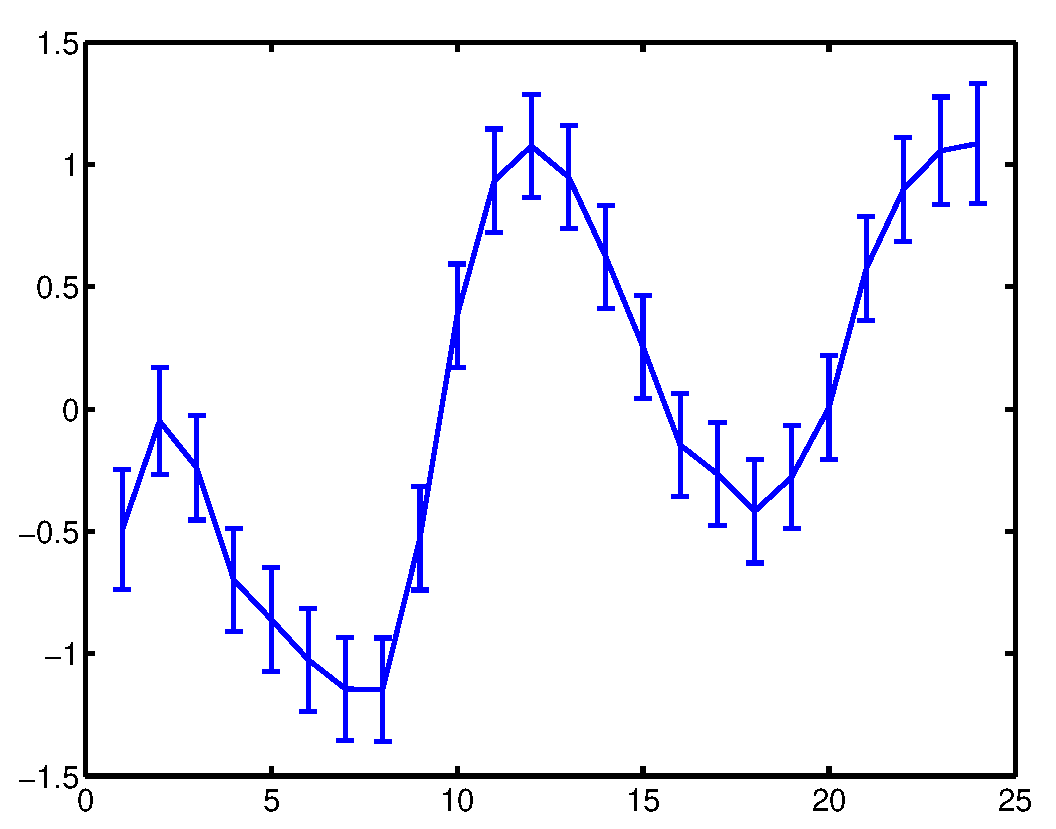
\includegraphics[%
%  width=1.8in,
% ]{/home/guido/mlprojects/chipChip/tex/figures/meanACE2errorbars.pdf}\vspace{-1.5cm}}
%\vspace{-1cm}\parbox{1.8in}{\center\scriptsize (a)}\nobreak\hspace{-0.6cm}\parbox{1.8in}{\center\scriptsize (b)}\vspace{-0.5cm}
%\parbox{1.8in}{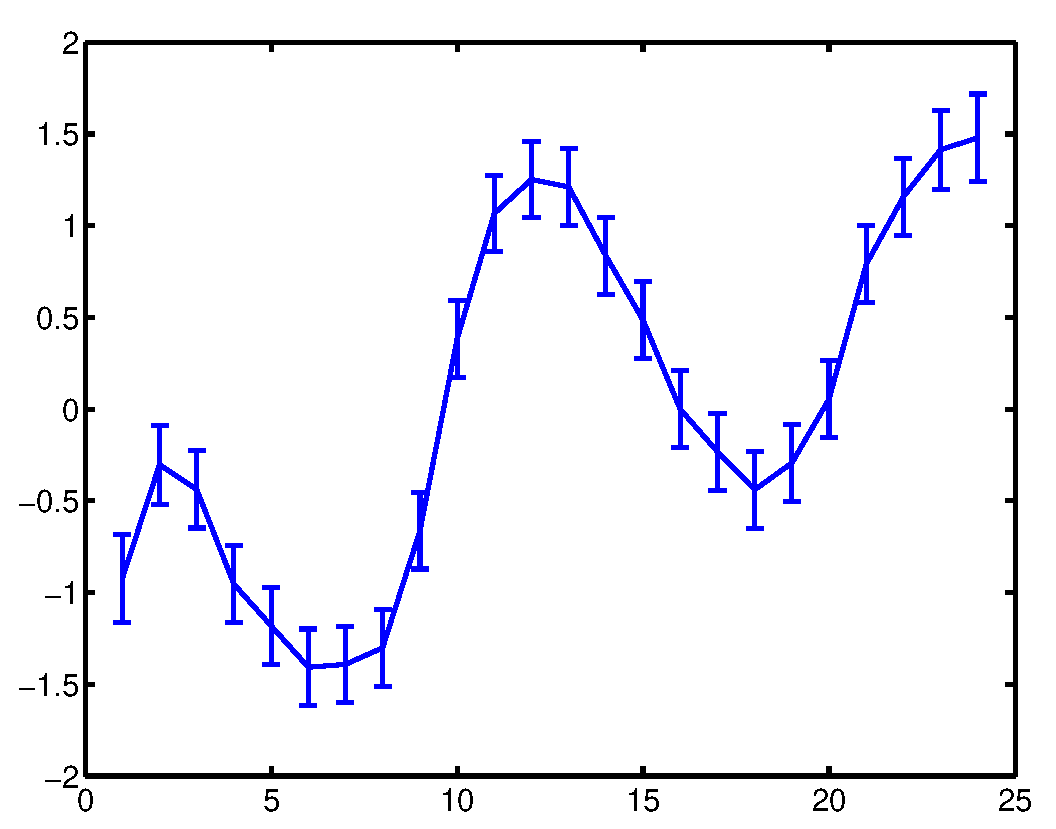
\includegraphics[%  
%width=1.8in]{/home/guido/mlprojects/chipChip/tex/figures/ACE2CTS1.pdf}\vspace{-1.5cm}}\nobreak\hspace{-1cm} 
%\parbox{1.8in}{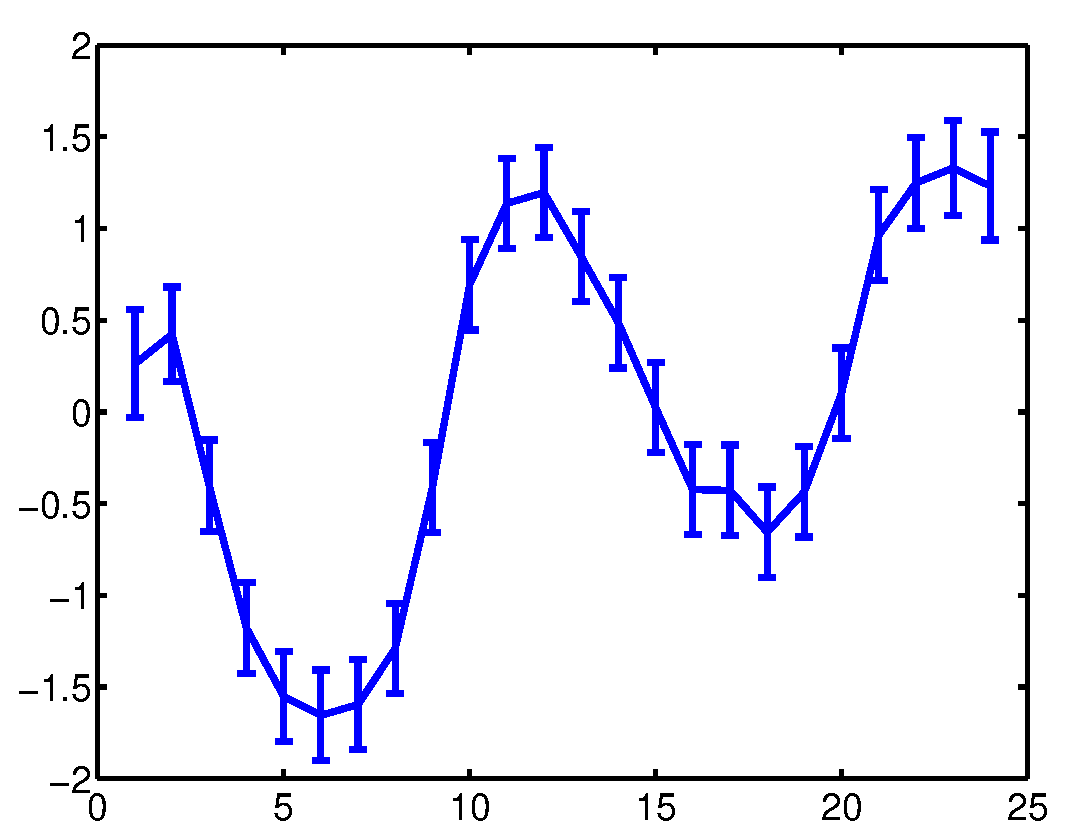
\includegraphics[%
%  width=1.8in,
%  ]{/home/guido/mlprojects/chipChip/tex/figures/ACE2SCW11.pdf}\vspace{-1.5cm}}
%\vspace{-1cm}\parbox{1.8in}{\center\scriptsize (c)}\nobreak\hspace{-0.6cm}
%\parbox{1.8in}{\center\scriptsize (d)} \vspace{0.5cm}
%{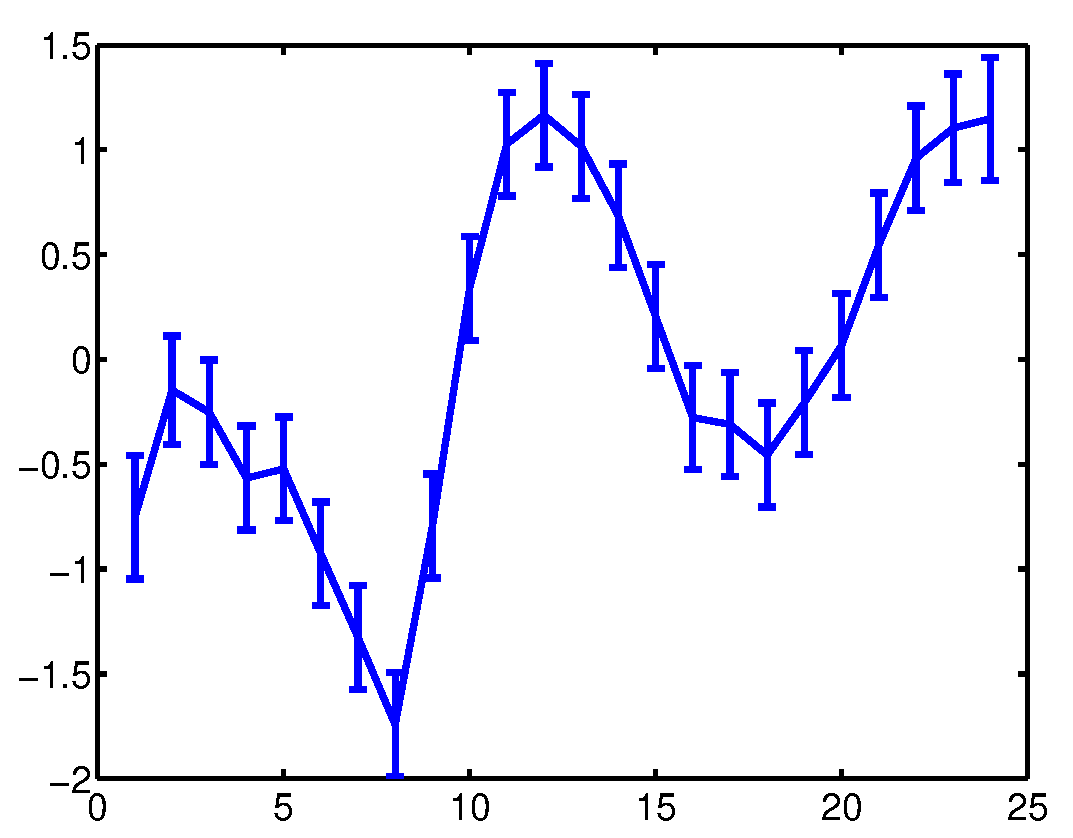
\includegraphics[%
%  width=0.50\columnwidth,
% ]{/home/guido/mlprojects/chipChip/tex/figures/ACE2YER124C.pdf}}{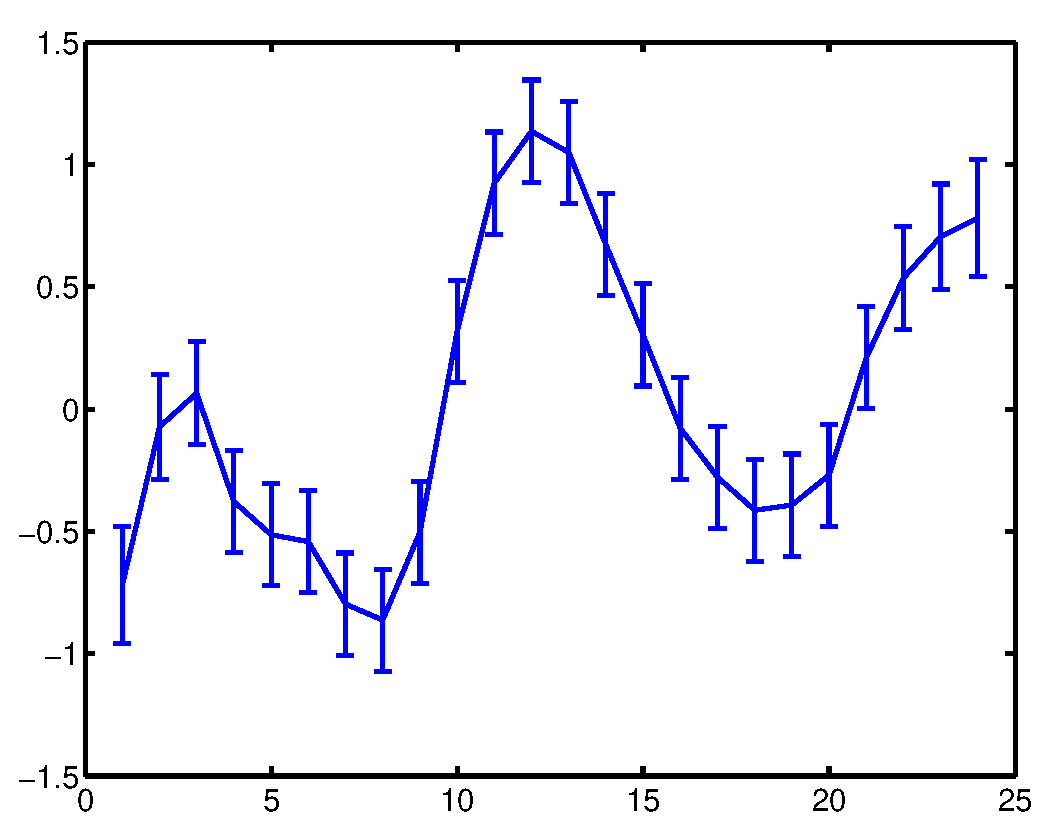
\includegraphics[%
%  width=0.50\columnwidth,
% ]{/home/guido/mlprojects/chipChip/tex/figures/ACE2YHR143W.pdf}}\vspace{-1cm}


\caption{TFAs and gene-specific TFAs of ACE2: (a) TFAs obtained by standard
multivariate regression (cf. \cite{Boule05}); (b) precision weighted mean of gene-specific TFAs 
for the four most significantly regulated genes; (c) TFA for gene YER124C  
and (d) TFAs for SCW11, the two genes with highest signal to noise ratio
in the gene-specific TFA.\label{cap:TFAs-and-gene-specific}}\vspace{-0.5cm}
\end{figure}
As well as providing a tool for identifying false positives in the connectivity
data, our model provides quantitative predictions on the strength of the 
regulatory activities through posterior estimation of the gene-specific TFAs.
As an example, we considered the posterior gene-specific TFAs for the 
well studied transcription factor ACE2. More examples can be found in the 
Supplementary Material.

ACE2 is predicted from ChIP experiments to bind to 59 different
genes. However, we found that \emph{a posteriori} the regulation was
significant only in 11 cases at a 95\% confidence level and in five cases
at 99\% confidence level. 
Three of the four most regulated genes, CTS1, 
YER124C and YHR143W, belong to one of the clusters identified by 
\citet{Spellman:yeastcellcy98}, the \emph{SIC1} cluster. 
Our results suggest that these genes 
are actually co-regulated and not only co-expressed. Their
qualitative behaviour, peaking at time point 11 in the M/G1 phase of the
cell cycle, is consistent
with the biological role of ACE2 in the cell cycle (see \cite{Spellman:yeastcellcy98}). TFA
profiles with error bars%
\footnote{Error bars are quite similar for different experimental points, but
not identical (even if the difference is hard to appreciate in
these figures).} for two of these genes are shown in Figure \ref{cap:TFAs-and-gene-specific}.
For comparison, we also show a precision-weighted average of the gene-specific
TFAs for the significantly regulated genes\footnote{The qualitative trend of 
the precision-weighted average across all targets of ACE2 is very similar to 
the one obtained considering only the most significantly regulated genes, but
the profile is more noisy.} and the TFA obtained by ordinary 
regression (see, for example, the similar figures in \cite{Boule05}). 
\subsubsection{Genes with multiple regulators}
When a gene is regulated by more than one transcription factor, it is possible
to use our model to determine \emph{a posteriori} the relative weight the 
different transcription factors play in regulating the gene. This can be done, 
for example, by ranking the transcription factors according to the maximum 
gene-specific TFA, and the significance level can then be assessed using the 
posterior variance.

The results of applying this procedure to some example genes 
are shown in Table \ref{cap:Relative-weight-of}.
The first two genes are two of the top four targets of  ACE2 described in the 
previous section, YER124C and YHR143W. We can see in these cases that the
activity of ACE2 explains the great majority of the expression of these two 
genes, and that the contribution of the other factors (FKH1 and FKH2) cannot be
considered statistically significant. The third row is an example of a gene 
which is significantly regulated by two transcription factors: while NDD1 
explains most of the expression of PHO3, a small but significant fraction is
attributed by our model to the action of FKH2. The situation appears different 
in the case of AGA1, a member of the \emph{MAT} cluster of genes involved in 
mating in the yeast cell \citep{Spellman:yeastcellcy98}. AGA1's expression
is chiefly explained by the activity of MBP1, but a significant role, both
statistically and quantitatively, is also played by SWI4, while MCM1's
contribution appears to
be insignificant.

At a more global level, one could consider patterns among the regulators of
genes that are significantly regulated by more than one transcription factor. 
The most represented pair of transcription factors is NDD1/FKH2 which 
significantly regulate six common target genes. This relationship is
confirmed in the literature \citep{Lee02}. Other relationships 
suggested by our model and documented in the literature are MBP1/FKH2, 
MBP1/SWI4 and MBP1/SKN7. A pair of transcription factors sharing three common
targets and not previously documented in the literature is DAL82/MTH1. 
Their shared targets are mostly low expressed genes, but
the model still assigns fairly high confidence to the prediction.

 

%
\begin{table}
\small\center\begin{tabular}{|>{\scriptsize}c|>{\scriptsize}c|}
\hline 
Gene name&
Regulators' activity\tabularnewline
\hline

\hline 
YER124C&
ACE2=1.1$\pm0.2$,
FKH2=0.03$\pm0.04$\tabularnewline
\hline 
YHR143W&
ACE2=1.4$\pm0.2$,
FKH2=0.03$\pm0.04$, FKH1=0.011$\pm0.009$\tabularnewline
\hline
PHO3&
NDD1=1.6$\pm0.2$,
FKH2=0.06$\pm0.02$\tabularnewline
\hline 
AGA1&
MBP1=1.5$\pm0.4$,
SWI4=1.0$\pm0.4$, MCM1=0$\pm0.003$\tabularnewline
\hline 
\end{tabular}
\vspace{0.2cm}

\caption{Four examples of genes regulated by multiple transcription factors.
The first two genes are effectively regulated only by ACE2, while the other
two genes genuinely have more than one active regulator\label{cap:Relative-weight-of}}
\vspace{-0.7cm}
\end{table}

\subsubsection{Correlations among transcription factors}\label{TransFact}
ACE2 was shown in \cite{Lee02} to be part of a group of eleven transcription 
factors which form an almost independent subnetwork in the cell cycle 
regulatory network. These are, besides ACE2: SWI4, SWI5, SWI6, STB1, MBP1,
SKN7, FKH1, FKH2, NDD1 and MCM1. 
We therefore expect correlations between these 
transcription factors to be particularly significant.

Correlations are captured by our model in several ways. The matrix $\Sigma$ 
models the \emph{a priori} covariance between transcription factors across 
genes, while 
posterior estimation can give insight into how correlated two transcription 
factors regulating the same gene are and how correlated TFAs are at 
different time points. 

To validate our model, we considered the normalised matrix of correlations $\hat\Sigma$ 
(the matrix $\Sigma$ with each entry divided by the standard deviation of the 
corresponding transcription factors). We considered the row of $\hat\Sigma$ 
corresponding to ACE2. This has \emph{a priori} 39 elements different from zero, as there are 
38 transcription factors that share at least one target gene with ACE2; 
however, most of these are very close to zero as the relevant transcription
factors do not significantly regulate any genes. We 
sorted them according to the absolute value of their correlation to ACE2, 
finding that 7 out of the 14 transcription factors most correlated with 
ACE2 are among the ten identified in \cite{Lee02}. Of these seven transcription
factors, two have large 
overlaps in their period of activity with ACE2 (SWI4 and MBP1), while two 
others (FKH2 and SWI5) are known to have important functional relationships
with ACE2. The remaining three (SKN7,FKH1 and NDD1) are known to coregulate genes
with FKH2 and 
probably their high correlation with ACE2 is obtained indirectly via the 
interaction with FKH2, rather than mirroring an actual interaction with ACE2. 


Of the remaining three transcription factors identified by \cite{Lee02},
but not identified by our model, 
MCM1 is active 
only during the inactive phase of ACE2, SWI6's period of activity is 
approximately a quarter of a period out of phase with ACE2's, and STB1 is 
active only  for a short interval approximately in the middle of the period of 
activity of ACE2, justifying a small correlation.

Some transcription factors were identified by our model as highly correlated 
with ACE2 even if they are not involved in the cell cycle. In some cases, 
there is an obvious biological link between these transcription factors and 
ACE2: YAP1, which is very positively correlated with ACE2, is known to be 
bound by ACE2 (\cite{Lee02}), while MSN4 is of the same functional type as ACE2
(zinc finger proteins). Also, it is possible that some transcription factors 
were active in other, collateral cellular processes which were taking place
simultaneously with the cell cycle: for example, YAP1 is known (\cite{Tu05}) to
be active at the peak of the oxidative phase in the metabolic cycle of the 
yeast cell, shortly before the cell cycle can take place. Correlation between
YAP1 and ACE2 could be supporting the hypothesis (\cite{Tu05}) that the 
metabolic cycle and the cell cycle can be coupled.

It is interesting to notice that, of the five transcription factors with highest 
correlation to ACE2, two have high positive correlations, FKH1 and FKH2 
(correlation 0.70 and 0.48 respectively), while three have large negative 
correlations, MBP1, SKN7 and SWI5 (correlation -0.59, -0.40 and -0.38 
respectively). This suggests that these transcription factors play 
complementary or opposite
roles in the regulation of their target genes, being active at mutually
excluding times or being promoter-repressor pairs. 
It would be interesting to validate experimentally
this prediction.

\subsection{Metabolic cycle data}
\cite{Tu05} investigated the molecular origin of the 
glycolitic and respiratory oscillations that constitute the yeast metabolic 
cycle. mRNA was prepared at regular intervals of approximately 25 minutes over 
three consecutive cycles. The study identified that, at 95\% significance, over
half of the yeast genes (approximately 3500) display periodic behaviour, and 
can hence be assumed to be metabolic cycle-regulated.

Raw data was processed with the multi-mgMOS algorithm of 
\cite{Liu:mmgmos05}, which provides uncertainties as well as expression levels 
for each gene and each experiment. We then used the modified model described 
in section \ref{uncertainty} to propagate these uncertainties through the 
estimation of gene-specific TFAs.

The connectivity data used  was recently obtained by 
\cite{Harbison04}, where the binding of 204 transcription factors to 6229 
genes during growth in rich medium was monitored. By removing genes not bound 
by any transcription factor 
and transcription factors not binding any gene, we reduced the size of the data
set to 2732 genes and 169 transcription factors.


\subsubsection{Active transcription factors} \cite{Tu05} 
provide a list of 133 transcription factors which display 
periodic behaviour in their expression levels at 95\% significance level. 
However, for all the reasons mentioned in the introductory section, it is 
doubtful whether periodicity in expression level can be considered strong
evidence as to whether a transcription factor is taking part in the regulation
of the metabolic cycle.

We therefore examined the gene-specific TFAs of all the 169 transcription 
factors actively binding targets, determining whether they significantly 
regulated any genes by examining signal to noise ratios. We obtained a list of
2410 regulatory relations involving 2167 genes and 151 transcription factors. 
We considered transcription factors regulating five or more genes and obtained
107 transcription factors which significantly regulated five or more genes. 
Sixty-six of these also 
belong to the list obtained in \cite{Tu05}. However, 41 transcription factors
which, according to our method, do significantly regulate periodic genes
do not have significantly periodic expression levels (see Supplementary 
Material).

For example, the zinc-finger transcription factor LEU3 is not included in the 
list of \cite{Tu05}; its expression profile, although approximately periodic,
is rather noisy (see Figure \ref{LEU3act} (a)). 
However, according to our method, it significantly 
regulates eight genes in the data set.
Five of these, 
OAC1, LEU1, BAT1,RPS11B and POL1, are highly periodic according to 
\citet{Tu05}. Three of these have recently been 
confirmed experimentally as targets of LEU3, and another 
significantly regulated (but non-periodic) gene, YOR271C, has been shown to be
bound by LEU3 \emph{in vitro} \citep{Boer05}.

These results indicate that LEU3 should be considered 
as a significant player in regulating the yeast metabolic cycle. Notice
that inference techniques which do not discriminate TFAs between 
genes would miss 
this fact: LEU3's average activity is indeed not periodic, as many of its 
targets are not periodic; only its 
gene-specific activity for some genes is periodic. Gene-specific TFAs 
of LEU3 in two periodic cases are shown in Figure \ref{LEU3act} (b)-(c). 
Figure \ref{LEU3act} (d) shows the gene-specific TFA of LEU3 acting on YGR190C.
Notice the  large error bars associated with the 
gene-specific TFA. YGR190C is, according to our model, a significantly 
regulated target of SWI4.    

A complete list of the active transcription factors and a comparison with the 
results of \citet{Tu05} is given in the Supplementary Material.

\begin{figure}
\setlength{\unitlength}{1cm} \begin{center}
    \begin{picture}(8,6) \epsfysize = 2.8cm
\epsfxsize=3.5cm
    \put(0,0){
\epsfbox{/home/guido/mlprojects/chipChip/tex/figures/LEU3BAT1.eps}}
      \put(3.0,-0.2){\mbox{\scriptsize{$t$}}}
    \put(-0.3,2.3){\mbox{\scriptsize{TFA}}} \put(1.9,-0.4){\mbox{(c)}}
\epsfxsize=3.5cm        \epsfysize =2.8cm \put(4.2,0){
\epsfbox{/home/guido/mlprojects/chipChip/tex/figures/LEU3YGR190C.eps}}
           \put(3.7 ,2.3){\mbox{\scriptsize{TFA}}}\put(5.9,-0.4){\mbox{(d)}}
        \put(7.1,-0.2){\mbox{\scriptsize{$t$}}} \epsfysize=2.8cm
\epsfxsize=3.5cm
    \put(0,3.3){
\epsfbox{/home/guido/mlprojects/chipChip/tex/figures/transcriptLEU3.eps}}
      \put(3.0,3){\mbox{\scriptsize{$t$}}}\put(1.9,2.9){\mbox{(a)}}
    \put(-0.3,5.8){\mbox{\scriptsize{$y$}}}
\epsfxsize=3.5cm        \epsfysize =2.8cm \put(4.2,3.3){
\epsfbox{/home/guido/mlprojects/chipChip/tex/figures/LEU3LEU1.eps}}
           \put(3.7 ,5.8){\mbox{\scriptsize{TFA}}}\put(5.9,2.9){\mbox{(b)}}
        \put(7.1,3){\mbox{\scriptsize{$t$}}}
         \end{picture} \end{center} 
\vspace{-0.2cm}
%\parbox{1.8in}{\includegraphics[width=1.8in,]
%{/home/guido/mlprojects/chipChip/tex/figures/transcriptLEU3.eps}\vspace{-1.5cm}}
%\nobreak \hspace{-1cm}\parbox{1.8in}{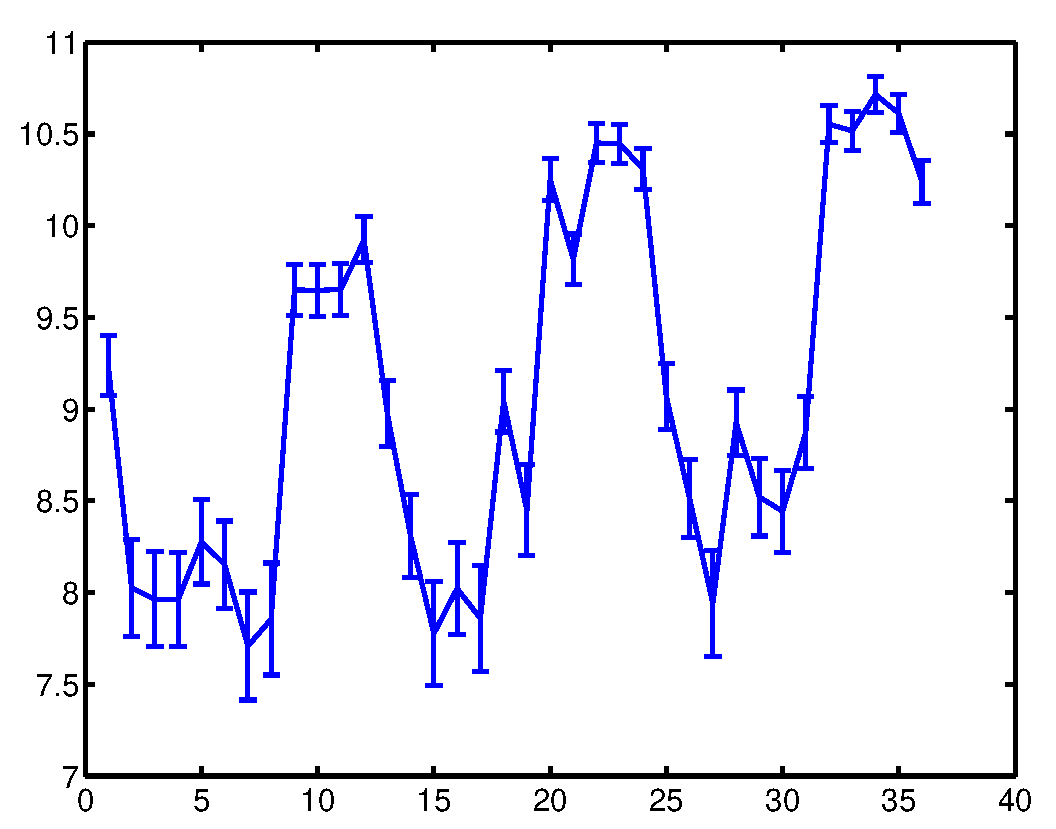
\includegraphics[%
%  width=1.8in,
% ]{/home/guido/mlprojects/chipChip/tex/figures/LEU3LEU1.eps}\vspace{-1.5cm}}
%\vspace{-1cm}\parbox{1.8in}{\center\scriptsize (a)}\nobreak\hspace{-0.6cm}\parbox{1.8in}{\center\scriptsize (b)}\vspace{-0.5cm}
%\parbox{1.8in}{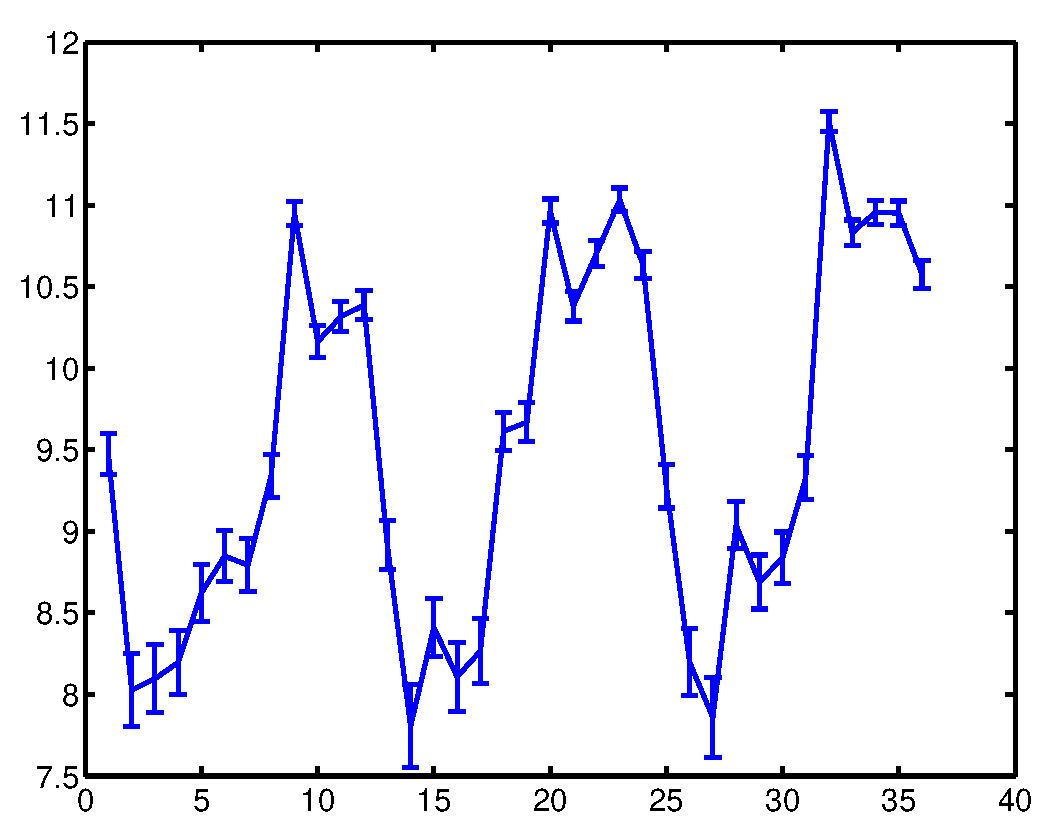
\includegraphics[%  
%width=1.8in]{/home/guido/mlprojects/chipChip/tex/figures/LEU3BAT1.eps}\vspace{-1.5cm}}\nobreak\hspace{-1cm} 
%\parbox{1.8in}{\includegraphics[%
%  width=1.8in,
%  ]{/home/guido/mlprojects/chipChip/tex/figures/LEU3RPS11B.eps}\vspace{-1.5cm}}
%\vspace{-1cm}\parbox{1.8in}{\center\scriptsize (c)}\nobreak\hspace{-0.6cm}
%\parbox{1.8in}{\center\scriptsize (d)} \vspace{0.5cm}%


\caption{(a) Expression profile for LEU3. Gene-specific TFAs of LEU3 acting on
(b) LEU1 and (c) BAT1. 
These genes were among a list of nine confirmed target genes 
identified by \cite{Boer05} using a comparison of various experimental 
techniques.(d) Gene-specific TFA of LEU3 acting on YGR190C, an example of a 
binding that doesn't result in significant regulation.
\label{LEU3act}}
\vspace{-0.6cm}
\end{figure}


\subsubsection{Comparison between metabolic and cell cycle data set}
One of the main features of our model is its environment specificity. Through 
its probabilistic nature, it can infer a different network structure in 
different experimental conditions. As an example, we again considered the 
transcription factor ACE2 and how it correlates to other transcription factors.

ACE2 is an active transcription factor in the metabolic cycle, both according
to our model and according to \cite{Tu05}. It significantly
regulates 14 genes, five of which are highly periodic according to \citet{Tu05}. 
However,
its list of significantly regulated targets is very different from the
list drawn from the cell cycle data: its four main targets are KRE32, 
YJR149W, YHL013C and LCP5. None of these was significantly regulated in the
cell cycle data set\footnote{It must be bourne in mind, though, that the 
ChIP data used was different. However, the same analysis conducted using the 
connectivity data of \cite{Lee02} highlights similar differences between the 
cell cycle and the metabolic cycle.}. 
Gene-specific TFAs for ACE2 on its most significantly 
regulated targets are shown in Figure \ref{ACE2met}. Notice that the two 
gene-specific TFAs are out of phase (correlation -0.5). It is hard to see 
how a regression method that assigns the same TFA to all target genes could 
have described this situation. 
\begin{figure}\vspace{-0.5cm}
\setlength{\unitlength}{1cm} \begin{center}
    \begin{picture}(8,3) \epsfysize = 2.8cm
\epsfxsize=3.5cm
    \put(0,0){
\epsfbox{/home/guido/mlprojects/chipChip/tex/figures/ACE2MRLP8.eps}}
      \put(3.0,-0.2){\mbox{\scriptsize{$t$}}}
    \put(-0.3,2.3){\mbox{\scriptsize{TFA}}}
\epsfxsize=3.5cm        \epsfysize =2.8cm \put(4.2,0){
\epsfbox{/home/guido/mlprojects/chipChip/tex/figures/ACE2UBR2.eps}}
       \put(7,-0.2){\mbox{\scriptsize{$t$}}}    \put(3.7 ,2.3){\mbox{\scriptsize{TFA}}}
\end{picture}\end{center}
\vspace{-0.5cm}
%{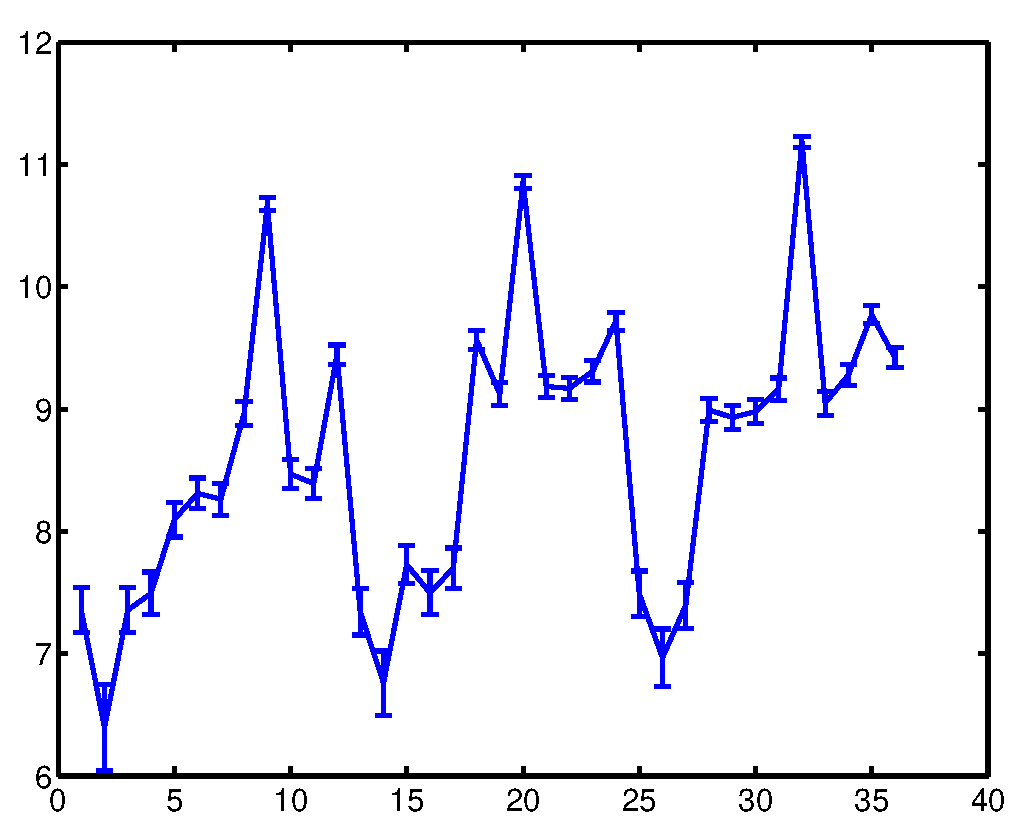
\includegraphics[
%  width=0.50\columnwidth,
%  keepaspectratio]{/home/guido/mlprojects/chipChip/tex/figures/ACE2MRLP8.eps}}{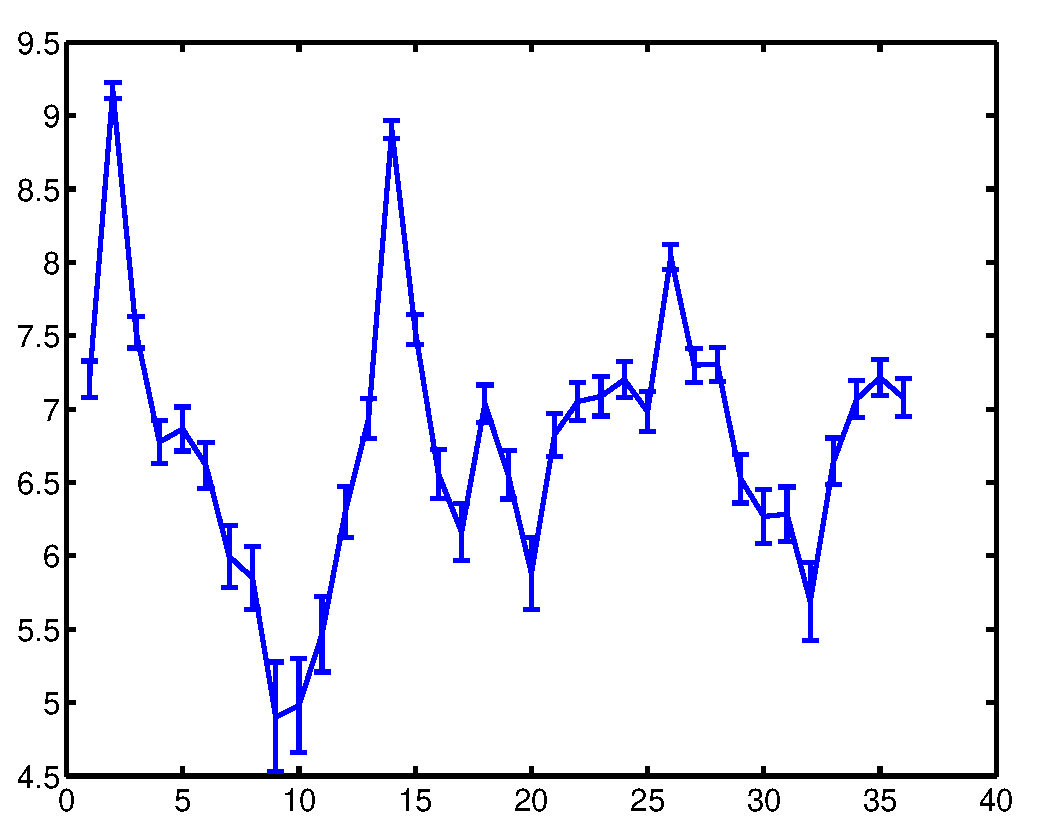
\includegraphics[%
%  width=0.50\columnwidth,
%  keepaspectratio]{/home/guido/mlprojects/chipChip/tex/figures/ACE2UBR2.eps}}
%\vspace{-2cm}



\caption{Gene-specific TFAs for ACE2 acting on KRE32 (\emph{left}) and YJR149W
(\emph{right}). \label{ACE2met}}\vspace{-0.5cm}
\end{figure}

We also examined the correlations between transcription factors predicted by 
our model in the metabolic cycle conditions. Again, the picture looks quite 
different from the cell cycle case: some correlations are similar, for example 
FKH2 is still positively correlated (correlation 0.62), 
while MBP1 is negatively correlated (correlation -0.53). However, some 
correlations which were negligible in the cell cycle data set appear to be more
important in the metabolic cycle. For example RME1, which was 
almost completely uncorrelated with ACE2 in the cell cycle data set, is 
now strongly positively correlated (correlation 0.50), 
while PHO4 and IME4 are now strongly negatively correlated (-0.46 and -0.51 
respectively). 

It would therefore seem that not only the structure of the regulatory network 
can change between different conditions, with some transcription factors 
changing their targets, but the way transcription factors work together can
change dramatically in different conditions. This is consistent with biological
knowledge, but, to our knowledge, our model is the first computational tool to
provide a genome-wide quantitative estimate of this change. 
\section{Discussion}

In this paper we introduced a novel probabilistic model for integrating
connectivity and microarray data. While most existing models infer trancription
factor activities that are shared across genes, we are able to infer
gene specific activities. The probabilistic nature of the model means
that we can associate credibility intervals with our results, and
hence determine which regulations are significant in a given experimental
condition.  

We validated our model on two yeast data sets, finding that the results of our 
model are in broad accordance with known biological facts about the yeast
transcriptional regulatory network. To demonstrate the flexibility of our 
model, we have shown how it can be used to answer a number of important
biological questions, such as: whether a transcription factor significantly 
regulates its target genes, what is the respective strength of transcription
factors co-regulating a gene? And what are the correlations among 
transcription factors? The ability to provide quantitative answers to these 
questions, 
while retaining a computational efficiency allowing genome-wide investigations,
is a unique feature of our model. It is a feature that we expect to be of great
assistance to biologists interested in the structure of regulatory
networks.

The model also provides new predictions that could shed light on some aspects
of the regulatory mechanism of the cell: for example, anticorrelation between 
transcription factors suggests mutually exclusive protein interactions, and 
negative gene-specific TFAs might be taken as a sign that the transcription
factor is repressing rather than promoting its target. These predictions could
hopefully be validated by new biological data in the future.

A common problem when using connectivity data is its notorious unreliability. 
The probabilistic nature of our model means that false positives have a reduced
influence on the results, as the model will associate them with high variances.
However, false negatives or incomplete data may still be problematic.
For example, it is possible that new transcription factors for yeast 
may be identified in the future \footnote{In the two years between 
\cite{Lee02} and \cite{Harbison04} 91 new transcription factors have been 
identified.}. Also, regulatory relationships are strongly environment dependent
and the use of ChIP data obtained in conditions even slightly different from 
the ones of the microarray data can result in many false negatives in the
connectivity data. This may lead to spurious 
results, as the model is forced to explain the effects of the unknown 
regulatory relations with the limited data available. There is no quick fix
to this problem: while we are investigating treating the connectivity data
as random variables, thus dealing with the associated uncertainty, it is
probable that the computational complexity will prove prohibitive in a
genome-wide application. For the time 
being, the best solution is to handle the results with some care, for example
requiring that a sufficient number of genes are significantly regulated by 
a transcription factor before concluding that that transcription factor is 
active in the given condition. Ultimately, the final arbiter should always be 
experimental biological validation.  
\section*{Acknowledgements}

We thank Balasz Papp, Stephen Oliver, Alastair Goldman and Marta Milo for 
useful discussions. We thank Andrzej Kudlicki for kindly making available
the CEL files for the yeast metabolic cycle data set, and Xuejun Liu for help 
using the mmgMOS package.
The authors gratefully acknowledge support from a BBSRC award {}``Improved
processing of microarray data with probabilistic models''. 
%\small\small


\bibliographystyle{abbrvnat}

\bibliography{chip}
\normalsize

\end{document}
